\documentclass{article}

\usepackage{Sweave}
\begin{document}
\input{tabgraf-concordance}

\begin{table}[h]
\centering
\caption{}
\begin{tabular}{l|r|r|r|r|r|r|r}
\hline
Parametri & min & q25 & median & q75 & max & mean & sd\\
\hline
Superficie (Kmq) & 1.97 & 10.6 & 17.1 & 29.2 & 227 & 29.8 & 43.9\\
\hline
Densità di popolazione (Ab/Kmq) & 4.02 & 45.1 & 128.1 & 257.1 & 2210 & 250.7 & 357.3\\
\hline
Altitudine mediana & 48.00 & 185.0 & 600.0 & 1120.0 & 2650 & 773.3 & 684.6\\
\hline
Superficie al pascolo (ettari) & 0.09 & 11.0 & 60.0 & 170.9 & 2630 & 178.8 & 338.8\\
\hline
Aziende con pascolo & 1.00 & 3.0 & 8.0 & 16.0 & 425 & 12.6 & 20.3\\
\hline
Capi al pascolo & 2.00 & 52.0 & 133.0 & 293.0 & 8429 & 307.1 & 602.7\\
\hline
\end{tabular}
\end{table}


\begin{table}[h]
\centering
\caption{}
\begin{tabular}{l|l|r|r}
\hline
Gruppo & SPECIE & n & prop\\
\hline
CERVIDI & CAPRIOLO & 201 & 70.53\\
\hline
CERVIDI & CERVO & 83 & 29.12\\
\hline
CERVIDI & DAINO & 1 & 0.35\\
\hline
BOVIDI & CAMOSCIO & 49 & 49.49\\
\hline
BOVIDI & MUFLONE & 44 & 44.44\\
\hline
BOVIDI & STAMBECCO & 6 & 6.06\\
\hline
CARNIVORI & TASSO & 5 & 20.83\\
\hline
CARNIVORI & VOLPE & 19 & 79.17\\
\hline
SUIDI & CINGHIALE & 78 & 100.00\\
\hline
LEPRE & LEPRE & 4 & 100.00\\
\hline
CORVIDI & CORNACCHIA & 133 & 88.67\\
\hline
CORVIDI & GAZZA & 13 & 8.67\\
\hline
CORVIDI & GHIANDAIA & 4 & 2.67\\
\hline
RAPACI & ALLOCCO & 3 & 4.41\\
\hline
RAPACI & ASSIOLO & 2 & 2.94\\
\hline
RAPACI & CIVETTA & 15 & 22.06\\
\hline
RAPACI & CIVETTA NANA & 1 & 1.47\\
\hline
RAPACI & FALCO PECCHIAIOLO & 7 & 10.29\\
\hline
RAPACI & GHEPPIO & 13 & 19.12\\
\hline
RAPACI & GUFO REALE & 4 & 5.88\\
\hline
RAPACI & NIBBIO BRUNO & 1 & 1.47\\
\hline
RAPACI & POIANA & 8 & 11.76\\
\hline
RAPACI & SPARVIERO & 14 & 20.59\\
\hline
UCCELLI ACQUATICI & CIGNO REALE & 3 & 20.00\\
\hline
UCCELLI ACQUATICI & CORMORANO & 1 & 6.67\\
\hline
UCCELLI ACQUATICI & FENICOTTERO & 1 & 6.67\\
\hline
UCCELLI ACQUATICI & FOLAGA & 1 & 6.67\\
\hline
UCCELLI ACQUATICI & GABBIANO & 1 & 6.67\\
\hline
UCCELLI ACQUATICI & GABBIANO REALE & 1 & 6.67\\
\hline
UCCELLI ACQUATICI & GERMANO REALE & 7 & 46.67\\
\hline
ALTRI VOLATILI & FAGIANO & 3 & 50.00\\
\hline
ALTRI VOLATILI & PICCIONE & 2 & 33.33\\
\hline
ALTRI VOLATILI & STARNA & 1 & 16.67\\
\hline
\end{tabular}
\end{table}

\begin{table}[h]
\centering
\caption{}
\begin{tabular}{l|r|r|r|r}
\hline
Specieagg & NM & P & T & Total\\
\hline
CERVIDI & 3 & 5 & 248 & 256\\
\hline
BOVIDI & 0 & 4 & 88 & 92\\
\hline
CARNIVORI & 5 & 0 & 15 & 20\\
\hline
SUIDI & 3 & 1 & 68 & 72\\
\hline
LEPRE & 1 & 0 & 2 & 3\\
\hline
CORVIDI & 118 & 1 & 19 & 138\\
\hline
RAPACI & 25 & 0 & 25 & 50\\
\hline
UCCELLI ACQUATICI & 3 & 3 & 6 & 12\\
\hline
ALTRI VOLATILI & 4 & 0 & 1 & 5\\
\hline
\end{tabular}
\end{table}

\begin{table}[h]
\centering
\caption{}
\begin{tabular}{l|r|r|r|r}
\hline
Specieagg & densPop alta & densPop media & densPop scarsa & Total\\
\hline
CERVIDI & 1 & 70 & 185 & 256\\
\hline
BOVIDI & 4 & 19 & 69 & 92\\
\hline
CARNIVORI & 0 & 6 & 14 & 20\\
\hline
SUIDI & 0 & 24 & 48 & 72\\
\hline
LEPRE & 0 & 1 & 2 & 3\\
\hline
CORVIDI & 1 & 58 & 79 & 138\\
\hline
RAPACI & 1 & 34 & 15 & 50\\
\hline
UCCELLI ACQUATICI & 3 & 6 & 3 & 12\\
\hline
ALTRI VOLATILI & 1 & 4 & 0 & 5\\
\hline
\end{tabular}
\end{table}


\begin{table}[h]
\centering
\begin{tabular}{l|r|r}
\hline
identificazione & n & prop\\
\hline
E.coli & 616 & 67.62\\
\hline
Klebsiella & 61 & 6.70\\
\hline
Enterobacter & 56 & 6.15\\
\hline
Serratia & 40 & 4.39\\
\hline
Pantoea & 39 & 4.28\\
\hline
Hafnia & 36 & 3.95\\
\hline
Proteus & 14 & 1.54\\
\hline
Acinetobacter & 13 & 1.43\\
\hline
Citrobacter & 12 & 1.32\\
\hline
Yersinia & 7 & 0.77\\
\hline
Cronobacter & 6 & 0.66\\
\hline
Salmonella & 5 & 0.55\\
\hline
Providencia & 4 & 0.44\\
\hline
Pseudomonas & 1 & 0.11\\
\hline
Shigella & 1 & 0.11\\
\hline
Total & 911 & 100.02\\
\hline
\end{tabular}
\end{table}

\begin{figure}[]
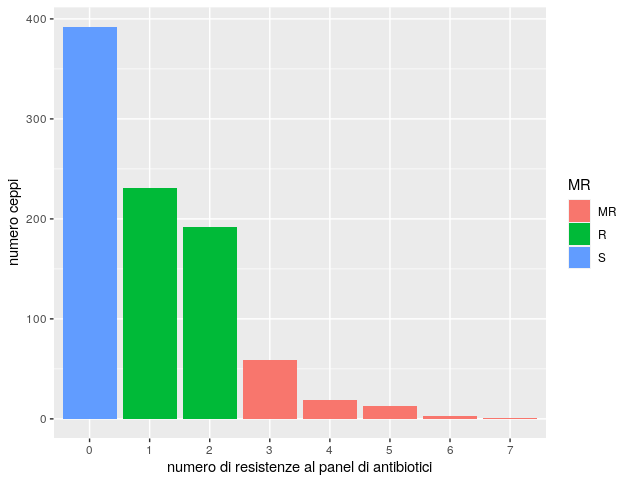
\includegraphics[width=1\linewidth]{figure/f1.png} \caption{}\label{fig:unnamed-chunk-1}
\end{figure}

\begin{figure}[]
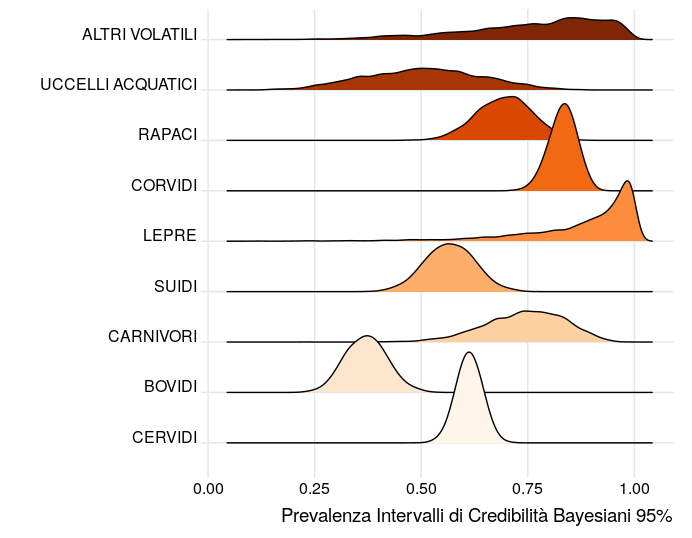
\includegraphics[width=1\linewidth]{figure/f3.png} \caption{}\label{fig:unnamed-chunk-1}
\end{figure}

\begin{figure}[]
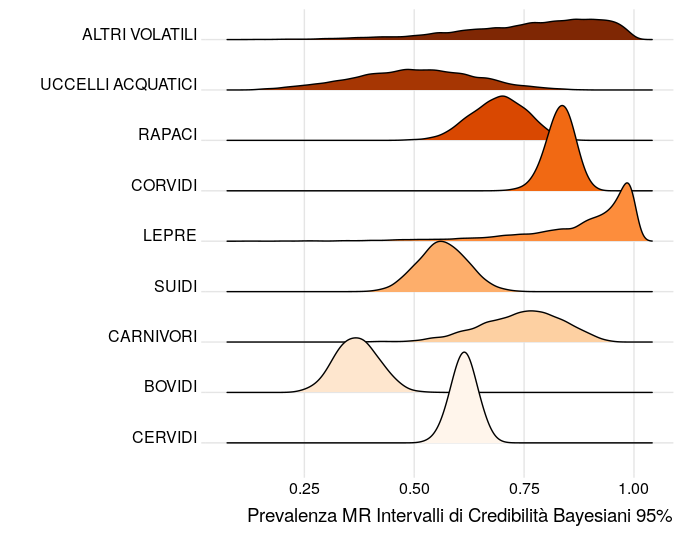
\includegraphics[width=1\linewidth]{figure/f4.png} \caption{}\label{fig:unnamed-chunk-1}
\end{figure}



\begin{table}[h]
\centering
\begin{tabular}{l|r|r|r}
\hline
antibiotico & R & S & \%Res\\
\hline
AMP & 392 & 531 & 42.5\\
\hline
TET & 342 & 581 & 37.0\\
\hline
CFT & 83 & 840 & 9.0\\
\hline
COL & 50 & 873 & 5.4\\
\hline
ENR & 46 & 877 & 5.0\\
\hline
KAN & 46 & 877 & 5.0\\
\hline
GEN & 12 & 911 & 1.3\\
\hline
\end{tabular}
\end{table}


\begin{figure}[]
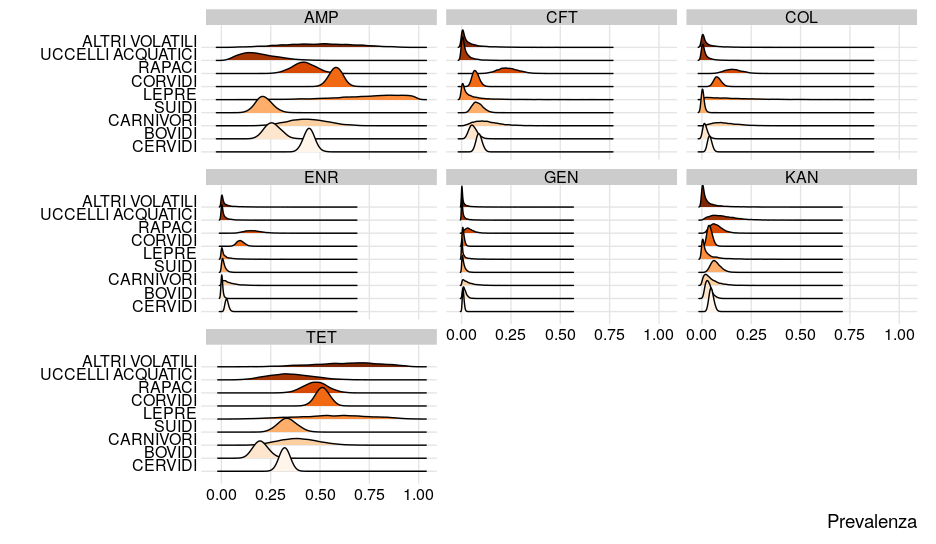
\includegraphics[width=1\linewidth]{figure/f5.png} \caption{}\label{fig:unnamed-chunk-1}
\end{figure}

\begin{figure}[]
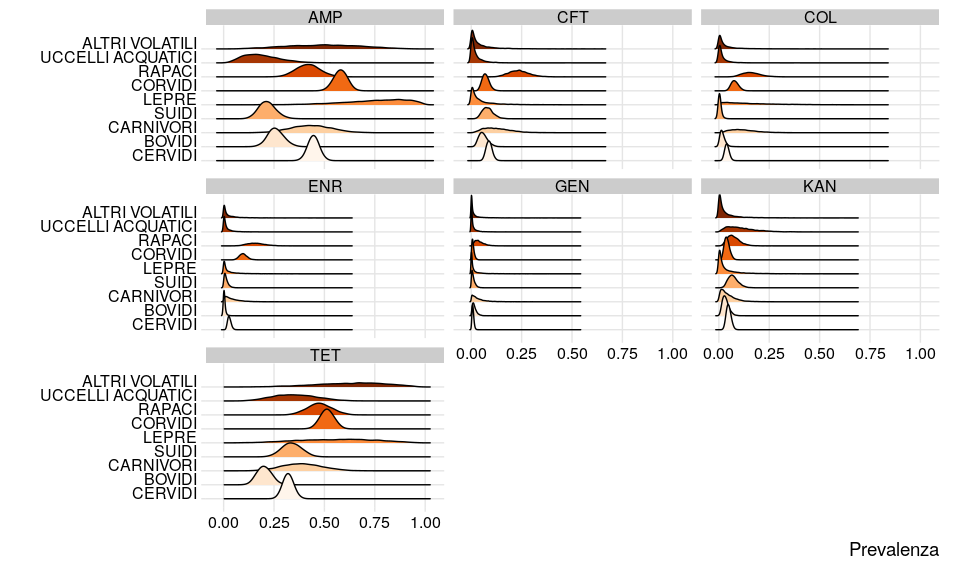
\includegraphics[width=1\linewidth]{figure/f6.png} \caption{}\label{fig:unnamed-chunk-1}
\end{figure}

\begin{table}[h]
\centering
\begin{tabular}{l|r|r|r|r|r|r|r}
\hline
Specieagg & AMP & CFT & COL & ENR & GEN & KAN & TET\\
\hline
CERVIDI & 0.45 & 0.09 & 0.04 & 0.03 & 0.01 & 0.05 & 0.32\\
\hline
BOVIDI & 0.26 & 0.06 & 0.02 & 0.00 & 0.02 & 0.03 & 0.20\\
\hline
CARNIVORI & 0.43 & 0.13 & 0.12 & 0.04 & 0.04 & 0.05 & 0.39\\
\hline
SUIDI & 0.22 & 0.08 & 0.00 & 0.01 & 0.01 & 0.07 & 0.34\\
\hline
LEPRE & 0.75 & 0.05 & 0.16 & 0.03 & 0.02 & 0.04 & 0.56\\
\hline
CORVIDI & 0.58 & 0.07 & 0.08 & 0.10 & 0.01 & 0.04 & 0.51\\
\hline
RAPACI & 0.42 & 0.24 & 0.16 & 0.16 & 0.04 & 0.07 & 0.48\\
\hline
UCCELLI ACQUATICI & 0.19 & 0.02 & 0.02 & 0.02 & 0.01 & 0.11 & 0.35\\
\hline
ALTRI VOLATILI & 0.50 & 0.05 & 0.04 & 0.03 & 0.02 & 0.04 & 0.63\\
\hline
\end{tabular}
\end{table}

\begin{table}[]
\centering
\begin{tabular}{l|r|r|r|r|r|r|r|r}
\hline
identificazione & tot & AMP & CFT & COL & ENR & GEN & KAN & TET\\
\hline
Acinetobacter & 13 & 84.62 & 76.92 & 7.69 & 30.77 & 0.00 & 0.00 & 23.08\\
\hline
Citrobacter & 12 & 66.67 & 0.00 & 0.00 & 16.67 & 0.00 & 8.33 & 41.67\\
\hline
Cronobacter & 6 & 66.67 & 0.00 & 0.00 & 16.67 & 0.00 & 0.00 & 16.67\\
\hline
E.coli & 616 & 32.47 & 9.42 & 2.92 & 4.06 & 1.30 & 6.49 & 34.90\\
\hline
Enterobacter & 56 & 87.50 & 0.00 & 7.14 & 5.36 & 1.79 & 1.79 & 67.86\\
\hline
Hafnia & 36 & 75.00 & 2.78 & 0.00 & 2.78 & 0.00 & 2.78 & 61.11\\
\hline
Klebsiella & 61 & 68.85 & 1.64 & 0.00 & 8.20 & 0.00 & 0.00 & 22.95\\
\hline
Pantoea & 39 & 15.38 & 0.00 & 2.56 & 0.00 & 0.00 & 0.00 & 5.13\\
\hline
Proteus & 14 & 14.29 & 21.43 & 100.00 & 0.00 & 14.29 & 7.14 & 100.00\\
\hline
Providencia & 4 & 0.00 & 0.00 & 100.00 & 0.00 & 0.00 & 0.00 & 25.00\\
\hline
Pseudomonas & 1 & 100.00 & 100.00 & 0.00 & 100.00 & 0.00 & 100.00 & 100.00\\
\hline
Salmonella & 5 & 100.00 & 0.00 & 20.00 & 0.00 & 0.00 & 0.00 & 80.00\\
\hline
Serratia & 40 & 72.50 & 7.50 & 15.00 & 7.50 & 2.50 & 0.00 & 55.00\\
\hline
Shigella & 1 & 100.00 & 0.00 & 0.00 & 0.00 & 0.00 & 0.00 & 0.00\\
\hline
Yersinia & 7 & 42.86 & 0.00 & 0.00 & 0.00 & 0.00 & 0.00 & 0.00\\
\hline
\end{tabular}
\end{table}

\begin{figure}[]
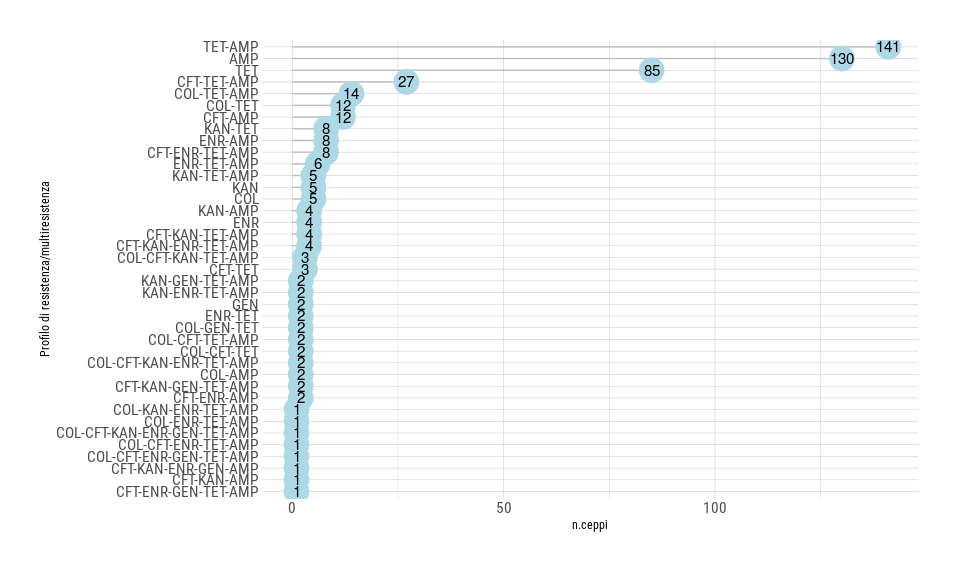
\includegraphics[width=1\linewidth]{figure/f7.png} \caption{}\label{fig:unnamed-chunk-1}
\end{figure}


\begin{figure}[]
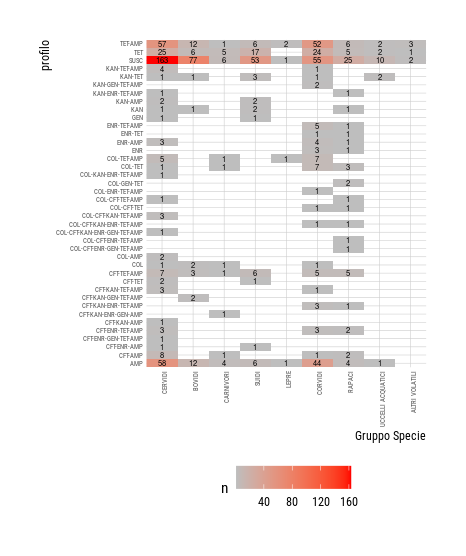
\includegraphics[width=1\linewidth]{figure/f8.png} \caption{}\label{fig:unnamed-chunk-1}
\end{figure}

\begin{table}[]
\centering
\begin{tabular}{l|r|r|r|r|r|r|r|r|r|r|r}
\hline
  & 0 & 0.25 & 0.5 & 1 & 2 & 4 & 8 & 16 & 32 & 64 & Inf\\
\hline
CERVIDI & 27 & 18.24 & 12.13 & 6.36 & 3.75 & 2.81 & 2.45 & 2.31 & 2.25 & 2.22 & 2.19\\
\hline
BOVIDI & 9 & 6.88 & 5.26 & 3.36 & 2.15 & 1.73 & 1.60 & 1.55 & 1.53 & 1.52 & 1.51\\
\hline
CARNIVORI & 10 & 9.24 & 8.51 & 7.28 & 5.76 & 4.75 & 4.27 & 3.98 & 3.82 & 3.74 & 3.67\\
\hline
SUIDI & 11 & 8.83 & 7.06 & 4.74 & 2.98 & 2.26 & 2.02 & 1.93 & 1.89 & 1.87 & 1.85\\
\hline
LEPRE & 4 & 3.95 & 3.90 & 3.79 & 3.57 & 3.20 & 2.84 & 2.66 & 2.57 & 2.54 & 2.50\\
\hline
CORVIDI & 22 & 16.75 & 12.85 & 8.49 & 5.89 & 4.94 & 4.55 & 4.35 & 4.22 & 4.14 & 4.05\\
\hline
RAPACI & 21 & 18.18 & 15.41 & 10.66 & 5.73 & 3.64 & 3.03 & 2.82 & 2.72 & 2.68 & 2.64\\
\hline
UCCELLI ACQUATICI & 5 & 4.57 & 4.16 & 3.44 & 2.56 & 2.03 & 1.83 & 1.76 & 1.73 & 1.71 & 1.70\\
\hline
ALTRI VOLATILI & 3 & 2.93 & 2.87 & 2.75 & 2.57 & 2.36 & 2.20 & 2.09 & 2.05 & 2.02 & 2.00\\
\hline
\end{tabular}
\end{table}

\begin{figure}[]
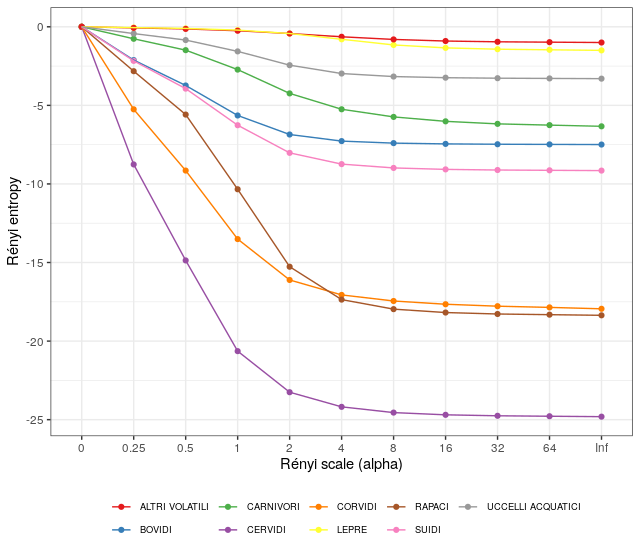
\includegraphics[width=1\linewidth]{figure/f9.png} \caption{}\label{fig:unnamed-chunk-1}
\end{figure}

\begin{table}[]
\centering\begin{table}

\centering
\begin{tabular}[t]{r}
\hline
x\\
\hline
728.4552\\
\hline
742.0757\\
\hline
776.3660\\
\hline
790.7783\\
\hline
799.5429\\
\hline
818.7644\\
\hline
\end{tabular}
\centering
\begin{tabular}[t]{r}
\hline
x\\
\hline
33.09793\\
\hline
18.62425\\
\hline
25.55846\\
\hline
31.33537\\
\hline
23.76134\\
\hline
36.04294\\
\hline
\end{tabular}
\centering
\begin{tabular}[t]{r}
\hline
x\\
\hline
0.00000\\
\hline
13.62051\\
\hline
47.91080\\
\hline
62.32315\\
\hline
71.08771\\
\hline
90.30924\\
\hline
\end{tabular}
\centering
\begin{tabular}[t]{r}
\hline
x\\
\hline
NA\\
\hline
25.07936\\
\hline
24.41350\\
\hline
21.24311\\
\hline
30.81553\\
\hline
19.65315\\
\hline
\end{tabular}
\centering
\begin{tabular}[t]{r}
\hline
x\\
\hline
89.702103\\
\hline
4.615869\\
\hline
5.774295\\
\hline
5.652207\\
\hline
5.621900\\
\hline
6.853777\\
\hline
\end{tabular}
\centering
\begin{tabular}[t]{r}
\hline
x\\
\hline
0.9988988\\
\hline
0.0011012\\
\hline
0.0000000\\
\hline
0.0000000\\
\hline
0.0000000\\
\hline
0.0000000\\
\hline
\end{tabular}
\end{table}
\end{table}

\end{document}
